\documentclass[12pt,a4paper]{article}

\usepackage[german]{babel}
\usepackage[utf8]{inputenc}
\usepackage[pdftex]{graphicx}
\usepackage{fancyhdr,lastpage}
\usepackage{enumerate}
\usepackage{amsmath, amsthm, amssymb}
\usepackage[top=3cm, bottom=3cm, left=2cm, right=2cm]{geometry}
\usepackage{minitoc}
\usepackage{multicol}
\pagestyle{fancy}

% Header
\lhead{Projekt Almond}
\chead{Abschlussbericht}
\rhead{Seite \thepage /\pageref{LastPage} }

\begin{document}

\begin{titlepage}
	\begin{center}
		
\includegraphics[height=15cm]{./logo.pdf}\\
		{\LARGE \bf Abschlussbericht}\\[0.3cm]
	\end{center}
\end{titlepage}

\tableofcontents

\newpage

% Inhalt

\section{Übersicht}
\subsection{Team}
Zunächst eine graphische Übersicht der Teammitglieder:\\
\begin{multicols}{2}{
\begin{list}{ }
	\item    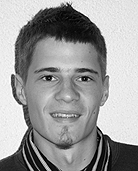
\includegraphics[height=1.5cm]{./face_Fanter.png}     \\      Stefan Profanter	
	\item    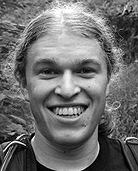
\includegraphics[height=1.5cm]{./face_Lotz.png}       \\      Linus Lotz 
	\item    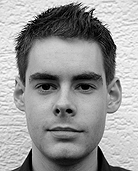
\includegraphics[height=1.5cm]{./face_Matthias.png}   \\      Matthias Schwab	
	\item    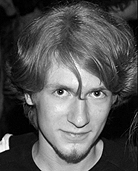
\includegraphics[height=1.5cm]{./face_Maxikay.png}    \\      Maximilian Karl
	\item    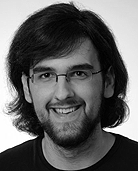
\includegraphics[height=1.5cm]{./face_Parsch.png}     \\      Thomas Parsch		
	\item 	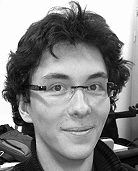
\includegraphics[height=1.5cm]{./face_Rupprecht.png}   \\      Christian Rupprecht
	\item    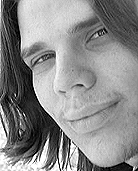
\includegraphics[height=1.5cm]{./face_Schnurrrr.png}  \\      Pascal Schnurr    
	\item    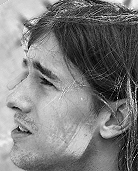
\includegraphics[height=1.5cm]{./face_Schon.png}      \\      Seán Labastille   
	\item    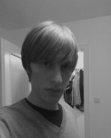
\includegraphics[height=1.5cm]{./face_Sickert.png}    \\      Salomon Sickert
\end{list}
}
\end{multicols}

\subsection{Infrastruktur}
Almond ({\bf A}utonomous {\bf L}ogging and {\bf M}anagement of {\bf N}etworked {\bf D}evices) ist ein Netzwerk aus unabhängigen Aktoren und Sensoren mit zentraler Überwachung und Steuerung.
Die Nuts ({\bf N}etworked {\bf Ut}ilities and {\bf S}ensors) sind Gruppierungen von Sensoren oder Aktoren. Diese werden über einen zentralen Controller (Squirrel) gesteuert. Zusätzlich gibt es ein Backend für PCs, welches über eine Weboberfläche Zugriff auf Gerätedaten gibt und die Steuerung der Aktoren sowie Konfigurationsänderungen erlaubt.\\
Die einzelnen Geräte werden über ein dafür entwickeltes Protokoll via Bluetooth mit dem Controller verbunden. Der Controller selbst wird dann ebenfalls über Bluetooth mit dem auf Linux, Windows oder Mac OS X laufenden Backend verbunden. Dabei werden auch Logdaten (Verlauf der Sensor-Werte) mit übermittelt, die dann später auf dem Rechner ausgewertet werden können.
\section{Komponenten}
\subsection{``Nuts''}
\begin{itemize}
	\item Entwurfsziele\\
	Eine Nut ist eine kompakte, kabellose Gruppierung von Sensoren und Aktoren mit möglichst niedrigem Stromverbrauch.
	\item Hardware\\
	Das Grundgerüst einer Nut bildet ein ATMega 8535 sowie eine Echtzeituhr und ein standardisiertes Bluetoothmodul welches auch auf der Suqirrel genutzt wird.
	\item Software\\
	Die Hauptaufgabe der in C entwickelten Software der Nut besteht darin die Sensorkalibrierung durchzuführen, Sensordaten auszulesen sowie per Downlink-Protokoll mit der Squirrel zu kommunizieren. Über Downlink können auch Befehle zum setzen von Aktoren empfangen werden.
\end{itemize}
\subsection{``Squirrel''}
\begin{itemize}
	\item Entwurfsziele\\
	Die Squirrel arbeitet als Autonome Kontrolleinheit mit der Aufgabe, die Log-Daten der Nuts auf SD-Karte zwischenzuspeichern und dem Backend bereitzustellen. Über ein integriertes Display (Emerging Display 13BB0) kann ein Menü angezeigt werden welches mit den 6 Steuerknöpfen gesteuert werden kann.
	\item Hardware\\
	Als Hauptprozessor dient ein XMega128A1. Das Board wurde selbst entwickelt und enhält einen SD-Kartenleser, eine Echtzeituhr (RTC) und ein Bluetoothmodul (BTM-222).
	\item Software\\
	Die Hauptaufgabe der Software, welche in C entwickelt wurde, dient zum Sammeln der Logdaten der Nuts und zum Übertragen der Logdaten an das Backend. Zusätzlich beinhaltet die Software den Display-/GUI-Treiber sowie einen FAT16-Treiber zum Speichern der Logdaten auf der SD-Karte.
\end{itemize}
\subsection{Backend}
\begin{itemize}
	\item Entwurfsziele\\
	Beim Backend handelt es sich um einen Plattformunabhängigen Server mit einer Webschnittstelle. Das Beckend dient zum Auslesen und Auswerten der Logdaten der Squirrel sowie zum Anzeigen von Log-Statistiken. Das Backend bietet zudem eine Übersicht über die Geräte und deren Status.
	\item Hardware\\
	Für das Backend wird ein Rechner mit Linux, Mac oder Windows benötigt, welcher über ein funktionierendes Bluetooth-Modul verfügen muss.
	\item Software\\
	Um Plattformunabhängigkeit zu erreichen wird für die Bluetooth-Kommunikation Java eingesetzt. Für das Webinterface wird Perl mit CGI verwendet, wodurch eine Integration in gängige Webserver gewährleistet wird. Für den Datenaustausch zwischen dem Java-Daemon und dem Webinterface dient eine MySQL-Datenbank.
\end{itemize}
\section{Umsetzung}
\subsection{Protokolle}
Um die Kommunikation zwischen den Nuts und der Squirrel, sowie der Squirrels zum Backend zu gewährleisten sind zwei Protokolle entworfen worden.\\
Die Protokollpakete sind folgendermaßen aufgebaut:
\\
\\
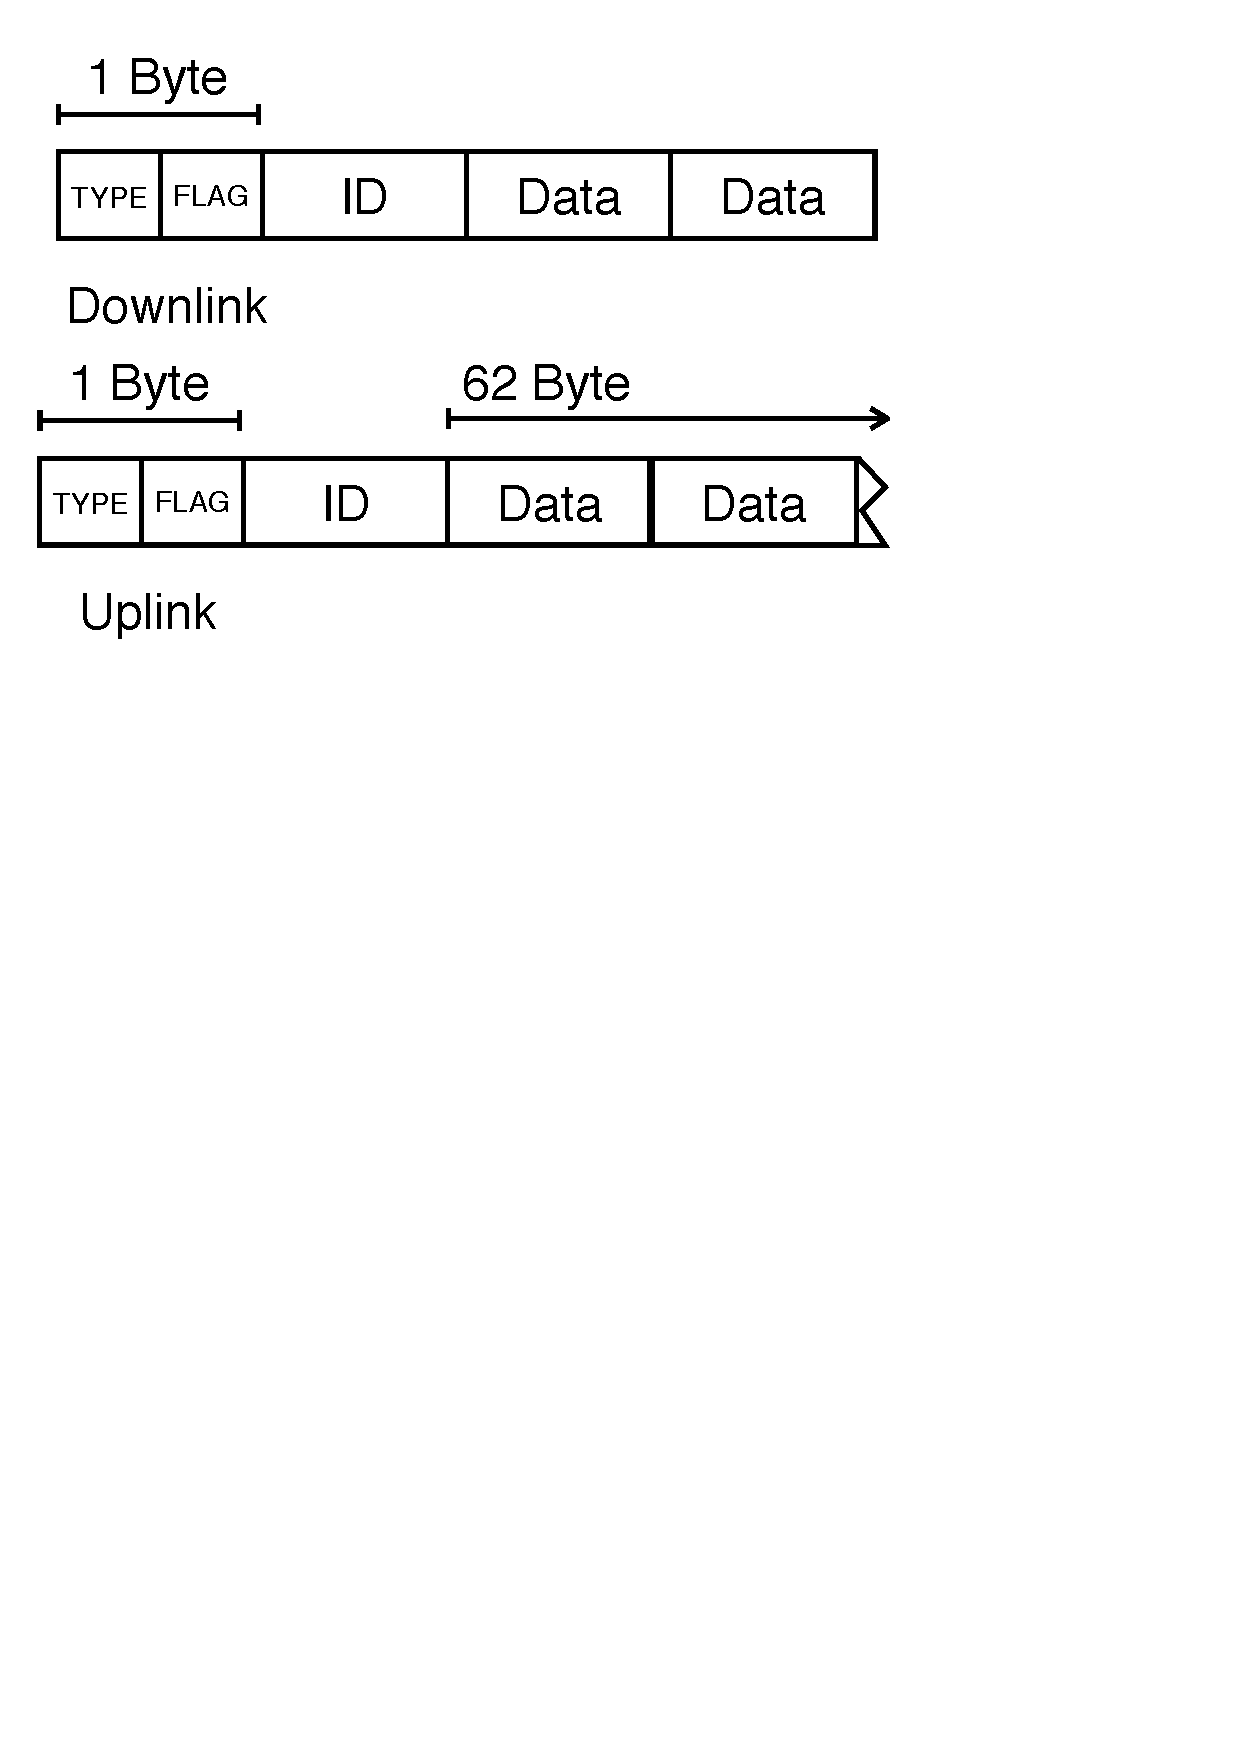
\includegraphics[height=6.5cm]{./ProkollDiagrams.pdf}\\

	\subsubsection{Downlink}  
Das Downlinkprotokoll dient zur Kommunikation der Nuts mit der Squirrel.\\
Im Protokoll sind folgende Befehle enthalten: SET, GET, ECHO, BYE\\
Durch die Reduzierung auf diese geringe Anzahl an Befehlen, wird eine sehr kleine Paketgröße von 4 Bytes erreicht.\\
Neben dem Opcode findet sich in einem Paket eine ID mit der Aktoren oder Sensoren angesprochen werden können. Sowie ein 16 Bit-Wert, der für Nutzdaten verwendet werden kann.\\
\begin{itemize}
	\item{SET}\\
Der SET-Befehl kann Aktoren auf bestimmte Werte setzen.
	\item{GET}\\
Der GET-Befehl liest die aktuellen Sensorwerte oder den Zustand eines Aktors aus.
	\item{ECHO}\\
Der ECHO-Befehl dient Debugging-Zwecken und sendet das empfangene Paket unverändert zurück.
	\item{BYE}\\
Der BYE-Befehl zeigt das Ende einer Verbindung an.
\end{itemize}
Um Variationen des GET-Befehls zu ermöglichen, wurden zusätzlich noch Flags implementiert.\\
\begin{itemize}
	\item{STANDARD}\\
Dieses Flag für die beeinflusst die Ausführung des Befehls nicht.
	\item{INFO\_NUT}\\
Dieses Flag dient dazu allgemeine - Sensor und Aktor unspezifische - Informationen der Nut, wie z.B. deren Namen abzurufen. Das übergebene ID-Feld wird nicht berücksichtigt.\\
	\item{INFO\_EXTENSION}\\
Mit diesem Flag werden Metadaten über den ausgewählten Sensor oder Aktor abgerufen.
\end{itemize}

	\subsubsection{Uplink}
Das Uplinkprotokoll dient zur Kommunikation zwischen der Squirrel und dem Backend.\\
Zum einen wird mit diesem Protokoll die Squirrel durch das Backend konfiguriert. Zum anderen kann das Backend Informationen über die aktuell verfügbaren Sensoren und Aktoren sowie deren Logdaten abrufen.\\
Es existieren folgende Befehle:
\begin{itemize}
	\item{LIST}\\
Teilt dem Backend alle verfügbaren Meta-Daten der Nuts, wie z.B. deren Bluetooth-Adresse, deren Sensoren und Aktoren, mit. Die Mess- und Zustandswerte selbst werden nicht übertragen.

	\item{LOG}\\
Mit diesem Befehle werden die in der Squirrel zwischengespeicherten Sensorwerte der verschiedenen Nuts dem Backend mitgeteilt.

	\item{TIME}\\
Mit diesem Befehl, kann das Backend die aktuelle Zeit der Squirrel mitteilen.

\end{itemize}
Hier folgt schematischer Kommunikationsablauf zwischen Backend, Squirrel und Nut:\\ 
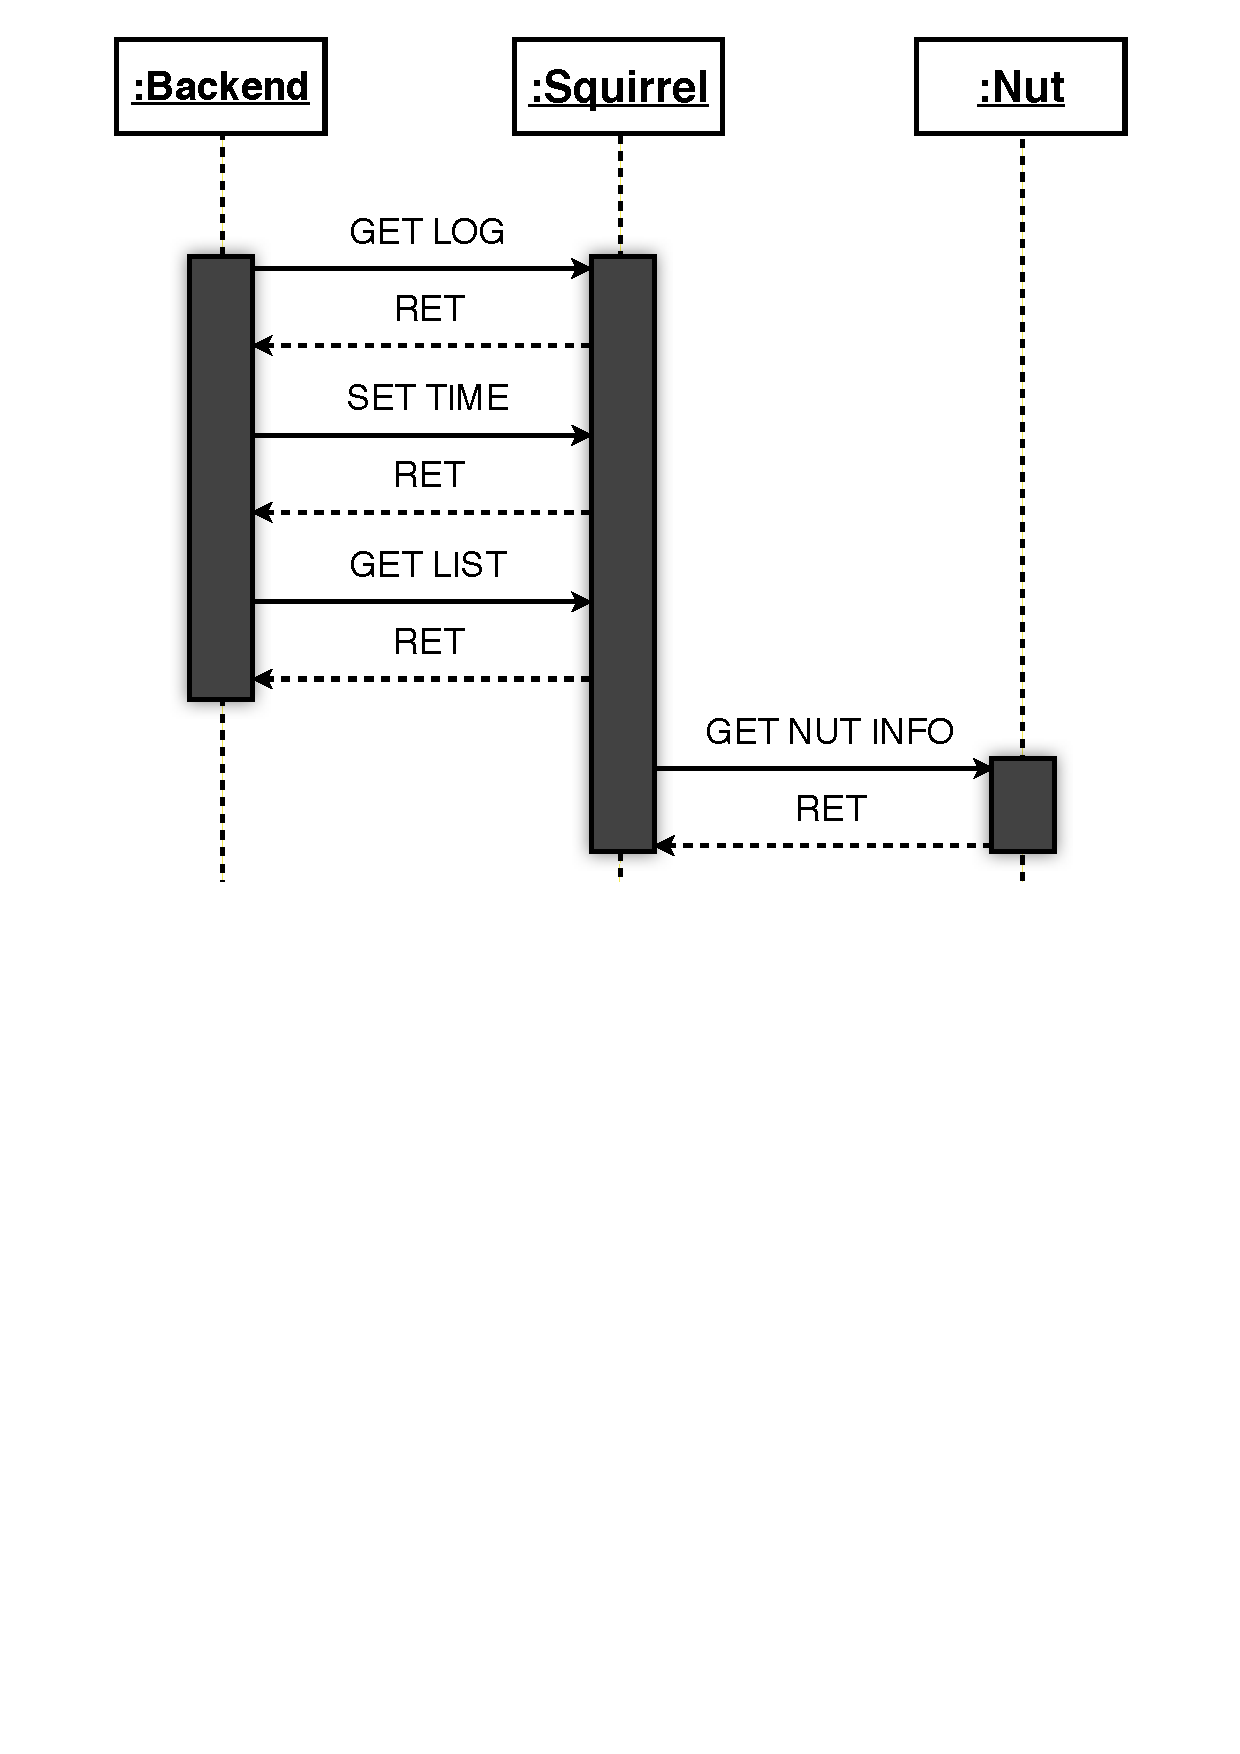
\includegraphics[height=8cm]{./ProtokollSequence.pdf}\\
\subsection{Embedded}
Die oben vorgestellten Protokolle stellen den Großteil des High-Level Interface zu dem Embedded-Teil von Almond. Als letzte wichtige High-Level-Komponente ist das Display zu erwähnen - auf dem eine möglichst komfortable Möglichkeit besteht direkt an der Squirrel einen Überblick über die vorhandenen Nuts und deren Zustand zu bekommen.\\
Diese Dienste basieren natürlich auf darunter liegende Hardwareschichten welche wir nun betrachten werden.\\
\subsubsection{Schnittstellen}
Auf Hardwareebene werden von den diversen Komponenten 3 Schnittstellen verwendet: SPI, I$^2$C sowie UART. Die GUI greift natürlich auf das Display zurück, wobei dieses nicht unbedingt als Schnittstelle im Sinne der gerade Aufgeführten gilt.\\
Kurz zu den Hardwareschnittstellen:
\begin{itemize}
	\item SPI\\
	Das Serial Peripheral Interface verfügt über 4 Pins, welche mit Master-Out-Slave-In (MOSI), Master-In-Slave-Out (MISO), CLOCK und Slave-Select (SS) bezeichnet werden.
	\begin{itemize}
	\item MOSI
	Der MOSI Pin stellt die Datenleitung vom Master zum Slave dar.
	\item MISO
	Der MISO Pin stellt die Datenleitung vom Slave zum Master dar.
	\item CLOCK
	Der Clock Pin ist der Anschluss der Taktleitung um die Taktfrequenz zu übertragen.
	\item SS
	Dient in diesem Projekt das Gerät zu aktivieren, da nur eines, die SD-Karte angeschlossen ist.
	\end{itemize}
	SPI wird zur Ansteuerung der SD-Karte genutzt.
	\item I$^2$C\\
	Über I$^2$C sind der Sensorchip der Nut (BMP085), sowie die Echtzeituhr der Squirrel angeschlossen.
	\item UART\\
	Universal Asynchronous Receiver/Transmitter - ein Übertragungsstandard für serielle Schnittstellen - wird im Almond-Projekt für die Anbindung der Bluetoothmodule sowohl auf der Nut als auch der Squirrel verwendet.
\end{itemize}
\subsection{Backend}
Das Backend stellt eine Web-Oberfläche zur Verfügung über die es möglich ist Log-Daten aus der Squirrel grafisch aufbereitet darzustellen oder Aktor-Befehle an die angeschlossenen Geräte zu senden. Das Backend besteht aus einem in Java geschriebenen Daemon sowie einer in Perl geschriebenen Web-Oberfläche die via CGI über einen Webserver verfügbar gemacht wird.

\subsubsection{Daemon}
Der Daemon ist ein in Java geschriebenes Programm, welches mit Hilfe der Bluecove-Libary die Aktivitäten des Squirrels - und somit des gesamten Almond-Systems - überwacht.\\
Die anfallenden Log-Daten werden in einer SQLite-Datenbank gespeichert.\\
Außerdem überprüft es in der Datenbank, ob mit Hilfe des Web-Interfaces Aktoren gesteuert werden. Ist dies der Fall, werden die entsprechenden Kommandos direkt über Bluetooth mit dem Downlinkprotokoll - unter Umgehung des Squirrels - an die Nuts gesendet.\\

\subsubsection{Datenbank}
Als Datenbank wird auf MySQL Server zurückgegriffen. Auf dem Backend-System welches den Webserver zur Verfügung stellt wird ein MySQL vorrausgesetzt das auch zur Kommunikation zwischen der Web-Oberfläche und dem Java-Daemon dient. \\
Das launch-Script des Backends liest Zugangsdaten und Schema-Name aus der Konfigurationsdatei und legt die benötigten Tabellen an.

\subsubsection{Web-Server}
Das Backend nutzt als Benutzeroberfläche eine in Perl geschriebene Web-Anwendung, was Nutzung von mehreren Web-Fähigen Geräten aus einfach macht. Die Web-Oberfläche kann als Virtual-Host in einen vorhandenen Webserver (z.B. Apache oder lighttpd) integriert werden. Vorraussetzung ist eine perl Runtime, einige Perl-Module (siehe README.txt im Backend) sowie ein CGI fähiger Webserver. Ist ein lighttpd auf dem Server-System installiert der nicht genutzt wird, kann das launch-Script diesen mit einer bereits vorkonfigurierten Datei starten und das Web-Interface läuft ohne weitere Modifikationen.
Das launch-Script des Backends startet auch den Java-Daemon, der über die MySQL Datenbank dann mit der Oberfläche kommuniziert.
\section{Stand}
\subsection{Wetterstation}
Die auf der im Rahmen des Projekts entwickelten Nut befindlichen Sensoren wurden zum Einsatz als ``Wetterstation'' gewählt.
Das ursprüngliche Vorhaben die Windrichtung zu messen wurde verworfen, es bleiben jedoch Möglichkeiten die Temperatur, Luftfeuchtigkeit, Luftdruck sowie die Helligkeit zu messen.
% FIXME Geht's jetzt?
\subsection{Status}
Aufgrund der erheblichen Widrigkeiten welche unter anderem bei der Nutzung des Bluetoothmoduls bestehen, ist die integrierte Nutzung der im einzelnen weitgehend funktionstüchtigen Komponenten nicht möglich. Es lassen sich jedoch in gewissem Umfang bestimmte Komponenten wie das Backend zur Auswertung der Logdaten, zu Zeitpunkten wo eine Datenübertragung per Bluetooth möglich ist, nutzen.

\end{document}
